\documentclass[a4paper]{scrreprt}
 
\usepackage[german]{babel}
\usepackage[utf8]{inputenc}
\usepackage[T1]{fontenc}
\usepackage{ae}
\usepackage[bookmarks,bookmarksnumbered]{hyperref}
\usepackage{graphicx}
 
\begin{document}
\title{Pflichtenheft für MensaMeet}

\maketitle
%\Footnote für Fußnoten
 
% Platzierung des Inhaltsverzeichnisses
\tableofcontents

\chapter{Motivation}

Wer kennt es nicht: Man ist an der Uni, die Freunde sind im Bett geblieben oder haben sich ein langes Wochenende gegönnt, deshalb sitzt man nun allein im Vorlesungssaal und überlegt was man nachher Essen möchte. Man schreibt Bekannte an. Möchte nicht jemand mit einem essen gehen? Aber Keiner ist da, Keiner hat Zeit. So muss man wohl mal wieder allein in die Mensa gehen. Dabei wäre nette Gesellschaft deutlich schöner. Man stellt sich in der Linienschlange an, lauscht den Gesprächen anderer. Am liebsten würde man mitreden. Aber einfach Fremde ansprechen und sich dazugesellen? Das käme doch komisch, oder? Aus dieser Situation entstand die Inspiration für MensaMeet. Mensameet ist viel mehr, als bloß ein Mensaplan. Man kann sich mit anderen Verabreden und neue Kontakte knüpfen. Die Zeiten des einsam Essens sind vorrüber!

\chapter{Zielbestimmung}
Mit dieser App sollen Personen(Studenten), die in der Mensa essen möchten, in die Lage versetzt werden, sich mit ihnen unbekannten Personen (Studenten) zum Essen verabreden zu können. Auf diese Art können leicht neue Menschen kennengelernt werden und keiner muss nicht alleine essen.
 
\section{Musskriterien}

\begin{addmargin}[25pt]{0pt} 
\hypertarget{mk10}{\textbf{/MK10/}} Erstellen und Bearbeiten eines persönlichen Profils, bestehdend aus: \\ Einem eindeutigen Nutzernamen, Alter, Geschlecht, Status (Student, Professor, Auszubildener, Schüler, Sonstiges), Motto)\\
\hypertarget{mk10}{\textbf{/MK10/}} Einsehen des Mensaplans des aktuellen Tages\\
\hypertarget{mk20}{\textbf{/MK20/}} Auswählen der Mensalinien/Mensawerke\\
\hypertarget{mk30}{\textbf{/MK30/}} Einsehen der Gruppen, mit übereinstimmenden Mensalnien/Werken\\
hypertarget{mk40}{\textbf{/MK40/}}Einstellen eines Zeitintervalls für das Essengehen \\
\hypertarget{mk50}{\textbf{/MK50/}} Erstellen einer Gruppe\\
\hypertarget{mk60}{\textbf{/MK60/}} Beitreten einer Gruppe\\
\hypertarget{mk70}{\textbf{/MK70/}} Verlassen einer Gruppe\\
\hypertarget{mk80}{\textbf{/MK80/}} Anschauen der Profile der Gruppenmitglieder\\
\hypertarget{mk90}{\textbf{/MK90/}} Automatisches Löschen der Gruppe am Ende des Tages, oder wenn letzes Mitglied austritt\\
\end{addmargin}

\section{Wunschkriterien}
Diese Kriterien sind nach Prioritäten geordnet, beginnend mit der höchsten Priorität.

\begin{addmargin}[25pt]{0pt} 
\hypertarget{wk10}{\textbf{/WK10/}} Bitmoji erstellen, welches als Profilbild angezeigt wird \\
\hypertarget{wk20}{\textbf{/WK20/}} Pushbenachrichtigungen (z.B. Erinnerung kurz vor dem Treffen) \\
\hypertarget{wk30}{\textbf{/WK30/}} Ranking System um die Zuverlässigkeit einer Person einzuschätzen \\ 
	hierzu können Gruppenmitglieder angeben, welche Personen zur Verabredung erschienen bzw. nicht erschienen sind\\
\hypertarget{wk40}{\textbf{/WK40/}} Administrator Sicht, Administratoren sollen Gruppen und Nutzer löschen könne\\
\hypertarget{wk50}{\textbf{/WK50/}} Filtermöglichkeiten der angezeigten Gruppen z.B. nach Treffzeitpunkt, aktuelle oder maximale Mitgliederanzahl \\
\hypertarget{wk60}{\textbf{/WK60/}} Die Möglichkeit Personen-Profile oder Gruppen zu melden\\
\hypertarget{wk70}{\textbf{/WK70/}} Einstellbare Restriktionen für den Gruppenbeitritt, z.b. nach Geschlecht, Studiengang, Rang, Alter \\
\hypertarget{wk80}{\textbf{/WK80/}} EErweiterte Profileinstellungen (Sprachen, Mag, Mag nicht, Vegetarier/Veganer, Unverträglichkeiten (Laktose, Gluten, ... ))\\
\hypertarget{wk90}{\textbf{/WK90/}} Bearbeiten der \hyperlink{label2}{Gruppenparameter} soll möglich sein, solange keine weitere Person beigetreten ist\\
\hypertarget{wk100}{\textbf{/WK100/}} E-Mail Verifizierung für die Registrierung\\
\hypertarget{wk110}{\textbf{/WK110/}} Einsicht in den Mensaplan der folgenden Tage\\
\hypertarget{wk120}{\textbf{/WK120/}} Erstellen einer Gruppe für folgende Tage\\
\hypertarget{wk130}{\textbf{/WK130/}} Achievment-System, erhaltene Achievments werden in der Gruppe angezeigt\\
\end{addmargin}
 
\section{Abgrenzungskriterien}

\begin{addmargin}[25pt]{0pt} 
\hypertarget{ak10}{\textbf{/AK10/}} Kein Hochladen und Aufnehmen von Bildern möglich.\\
\hypertarget{ak20}{\textbf{/AK20/}} Entfernen von Personen aus einer Gruppe ist nicht möglich.\\
\hypertarget{ak30}{\textbf{/AK30/}} Es wird kein Chatsystem implementiert\\
\hypertarget{ak40}{\textbf{/AK40/}} Kein manuelles Löschen von Gruppen, außer durch Administratoren.\\
\hypertarget{ak50}{\textbf{/AK50/}} Die App ist nur in deutscher Sprache verfügbar und nicht barrierefrei. \\
\end{addmargin}


\chapter{Produkteinsatz}
Das Produkt wird von Mensabesuchern eingesetzt, um sich mit unbekannte Personen zum gemeinsamen Essen in der Mensa zu verabreden.

 
\section{Anwendungsbereiche}
Die App wird für die \hyperlink{label3}{Essensplanung} an der Mensa eingesetzt.
 
\section{Zielgruppen}
\hyperlink{label1}Mensabesucher
 
\section{Betriebsbedingungen}
\subsection{Physikalische Umgebung}
Die App kann überall eingesetzt werden, wo das Smartphone Internetzugang hat,
z.B.: Zuhause, auf dem Campus, in geschlossen Räumen, in der Stadt, in der Straßenbahn

\subsection{Tägliche Betriebszeit}
Es wird erwartet, dass ein Nutzer die App bis zu 3 mal täglich verwendet. \\
Die erwartete Nutzungsdauer am Stück beträgt maximal 10 Minuten. 
 
\chapter{Produktumgebung}
Das Produkt läuft als App auf einem Smartphone.

\section{Software}
Android Version 4.4 oder höher.
 
\section{Hardware}
Smartphone 
 
\chapter{Funktionale Anforderungen}
TODO Sie werden eingeteilt in Client und Server Funktionalitäten.

\section{Client}
Auf dem Client (in diesem Fall ein Smartphone) müssen alle folgende Anforderungen erfüllt sein. 

\subsection{Allgemein}

\begin{addmargin}[25pt]{0pt} 
\textbf{/CAFA10/} Installation der Applikation \\
\textbf{/CAFA20/} Starten / Beenden der Applikation\\
\textbf{/CAFA30/} Speicherung lokaler Daten (Login Daten)\\
\end{addmargin}

\subsection{User Interface}

\begin{addmargin}[25pt]{0pt} 
\hypertarget{cifa10}{\textbf{/CIFA10/}} Anmelden / Registrieren \\
Es muss eine Seite geben auf der Buttons für Anmeldung und Registrierung sind.
\hypertarget{cifa20}{\textbf{/CIFA20/}} Angaben persönlicher Daten (\hyperlink{mk10}{MK10})\\
\hypertarget{cifa30}{\textbf{/CIFA30/}} Anzeigen und Auswählen der Essenslinien\\
\hypertarget{cifa40}{\textbf{/CIFA40/}} Angeben des bevorzugten Zeitraums\\
\hypertarget{cifa50}{\textbf{/CIFA50/}} Anzeigen und Auswählen einer Gruppe\\
\hypertarget{cifa60}{\textbf{/CIFA60/}} Anzeigen eines Userprofils\\
\hypertarget{cifa70}{\textbf{/CIFA70/}} Anzeigen des Regelwerks\\
\hypertarget{cifa80}{\textbf{/CIFA80/}} Anzeigen der Gruppenseite\\
\hypertarget{cifa90}{\textbf{/CIFA90/}} Einstellngen des Profils\\
\end{addmargin}

\section{Server}

\begin{addmargin}[25pt]{0pt} 
\hypertarget{sfa10}{\textbf{/SFA10/}} User anlegen / löschen\\
\hypertarget{sfa20}{\textbf{/SFA20/}} User anmelden / abmelden\\
\hypertarget{sfa30}{\textbf{/SFA30/}} Gruppe erstellen mit Parametern\\
\hypertarget{sfa40}{\textbf{/SFA40/}} Gruppe löschen\\
	\begin{addmargin}[25pt]{0pt} 
	\hypertarget{sfa41}{\textbf{/SFA41/}} Durch Autretten des letzten Users\\
	\hypertarget{sfa42}{\textbf{/SFA42/}} Durch Admin\\
	\hypertarget{sfa43}{\textbf{/SFA43/}} Automatisch durch Timeout\\
	\end{addmargin}
\hypertarget{sfa50}{\textbf{/SFA50/}} Anzeigen der Gruppen zu Parametern\\
\hypertarget{sfa60}{\textbf{/SFA60/}} User tritt Gruppe bei\\
\hypertarget{sfa70}{\textbf{/SFA70/}} User verlässt Gruppe\\
\hypertarget{sfa80}{\textbf{/SFA80/}} Informationen bearbeiten von User\\
\hypertarget{sfa90}{\textbf{/SFA90/}} Abfragen der Mensapläne\\
\hypertarget{sfa100}{\textbf{/SFA100/}} Abfragen von Userprofil\\
\end{addmargin}

\chapter{Produktdaten}

\section{Benutzerdaten}

\begin{addmargin}[25pt]{0pt}
\hypertarget{d10}{\textbf{/D10/}} Über einen Benutzer der App sind folgende Daten zu speichern:\\
Benutzername, Passwort, E-Mail (\hyperlink{wk20}{WK20}), Alter, Profilbild oder Bitmoji(\hyperlink{wk30}{WK30}), Motto, Geschlecht, Status (Student, Prof., Sonstiges), Essenspräferenzen, Administratorfunktionen (Ja/Nein)\\
\hypertarget{d20}{\textbf{/D20/}} Handelt es sich um einen Benutzer des Status Student, so ist zusätzlich der Studiengang zu erfassen\\
\hypertarget{d30}{\textbf{/D30/}} Erstellt ein Benutzer eine Gruppe, so wird diese Gruppe für Benutzerstatistiken und mögliche Ränge gespeichert\\
\hypertarget{d40}{\textbf{/D40/}}Tritt ein Benutzer einer Gruppe bei, so wird dies für Benutzerstatistiken gespeichert\\
\hypertarget{d50}{\textbf{/D50/}}Tritt ein Benutzer aus einer Gruppe aus, wird dies ebenfalls für Benutzerstatistiken gespeichert\\


\end{addmargin}

\section{Gruppendaten}

\begin{addmargin}[25pt]{0pt}
\hypertarget{d60}{\textbf{/D60/}} Über jede erstellte Gruppe sind folgende Daten zu speichern:\\
Gruppenname, Motto, Essenslinie, Uhrzeit, Teilnehmeranzahl, Ersteller, Gruppenmitglieder\\
\end{addmargin}

\section{Mensadaten}

\begin{addmargin}[25pt]{0pt}
\hypertarget{d70}{\textbf{/D70/}} Die zu speichernden Mensadaten beinhalten lediglich den tagesaktuellen Speiseplan\\
\end{addmargin}



\chapter{Nichtfunktionale Anforderungen}

\begin{addmargin}[25pt]{0pt} 

\hypertarget{nfa10}{\textbf{/NFA10/}} Es können bis zu 10.000 User in der Datenbank angelegt werden.\\
\hypertarget{nfa20}{\textbf{/NFA20/}} Eingaben dürfen nicht länger als 255 Zeiche sein.\\
\hypertarget{nfa30}{\textbf{/NFA30/}} Benutzernamen dürfen nicht länger als 40 Zeiche sein.\\
\hypertarget{nfa40}{\textbf{/NFA40/}} Es können beim Suchen passender Gruppen bis zu 24 Ergebnisse geliefert werden, um die Serverauslastung zu minimieren.\\
\hypertarget{nfa50}{\textbf{/NFA50/}} Serverarbeiten fidnen nur zwischen 0:00 und 6:00 Uhr statt.\\
\hypertarget{nfa60}{\textbf{/NFA60/}} Das System muss parallel von bis zu 1000 Usern benutzt werden können.\\
\hypertarget{nfa70}{\textbf{/NFA70/}} Das System darf nicht mehr als einen Neustart pro Woche brauchen.\\
\hypertarget{nfa80}{\textbf{/NFA80/}} Es soll ab Öffnen der App in 6 Klicks möglich sein einer Gruppe beizutreten .\\
\hypertarget{nfa90}{\textbf{/NFA90/}} Alle Buttons sollen gut lesbar und leicht anklickbar sein.\\

\end{addmargin}


\chapter{Globale Testfälle}

\begin{addmargin}[25pt]{0pt} 
\hypertarget{t10}{\textbf{/T10/}} Ein nicht registrierter Nutzer öffnet die App, registriert sich erfolgreich und gelangt auf die „Profil Bearbeiten“-Seite\\
  \begin{addmargin}[25pt]{0pt} 
  \hypertarget{t11}{\textbf{/T11/}} Bearbeitet dieser sein Profil vollständig, ist der Registrierungsprozess abgeschlossen und ihm stehen alle Benutzerfunktionen zur Verfügung\\
  \hypertarget{t12}{\textbf{/T12/}} Schließt dieser vorzeitig die Applikation, so wird er beim erneuten Öffnen direkt zur Profilbearbeitung weitergeleitet. Wiederholen bis erfolgreich abgeschlossen.\\
  \end{addmargin}
\hypertarget{t20}{\textbf{/T20/}} Ein registrierter Nutzer öffnet die App und betrachtet die Essenmöglichkeiten des aktuellen Tages\\
\hypertarget{t30}{\textbf{/T30/}} Ein Benutzer wählt eine Essenslinie und Uhrzeit aus und tritt anschließend einer der vorgeschlagenen Gruppen bei\\
  \begin{addmargin}[25pt]{0pt} 
  \hypertarget{t31}{\textbf{/T31/}} Erfolgreiche Teilnahme am Gruppentreffen\\
  \hypertarget{t32}{\textbf{/T32/}} Vorzeitiger Austritt aus der Gruppe und das anschließenden Anzeigen der Homeseite\\
  \end{addmargin}
\hypertarget{t40}{\textbf{/T40/}}  Erstellungsprozess einer Gruppe\\
  \begin{addmargin}[25pt]{0pt} 
  \hypertarget{t41}{\textbf{/T41/}} Erfolgreiche Erstellung durch Eingabe aller erforderlichen Daten\\
  \hypertarget{t42}{\textbf{/T42/}} Absichtlicher Abbruch des Erstellungsprozess\\
  \hypertarget{t43}{\textbf{/T43/}} Erstellung wird durch fehlende Parameter nicht beendet\\
  \end{addmargin}
\hypertarget{t50}{\textbf{/T50/}} Ein Administrator öffnet die App und gelangt auf die Adminseite\\
  \begin{addmargin}[25pt]{0pt} 
  \hypertarget{t10}{\textbf{/T51/}} Administrator löscht Gruppe\\
  \hypertarget{t10}{\textbf{/T52/}} Administrator löscht Benutzer\\
  \end{addmargin}



\end{addmargin}

\chapter{Systemmodelle}
\section{Anwendungsfalldiagramm}	

\begin{center}
	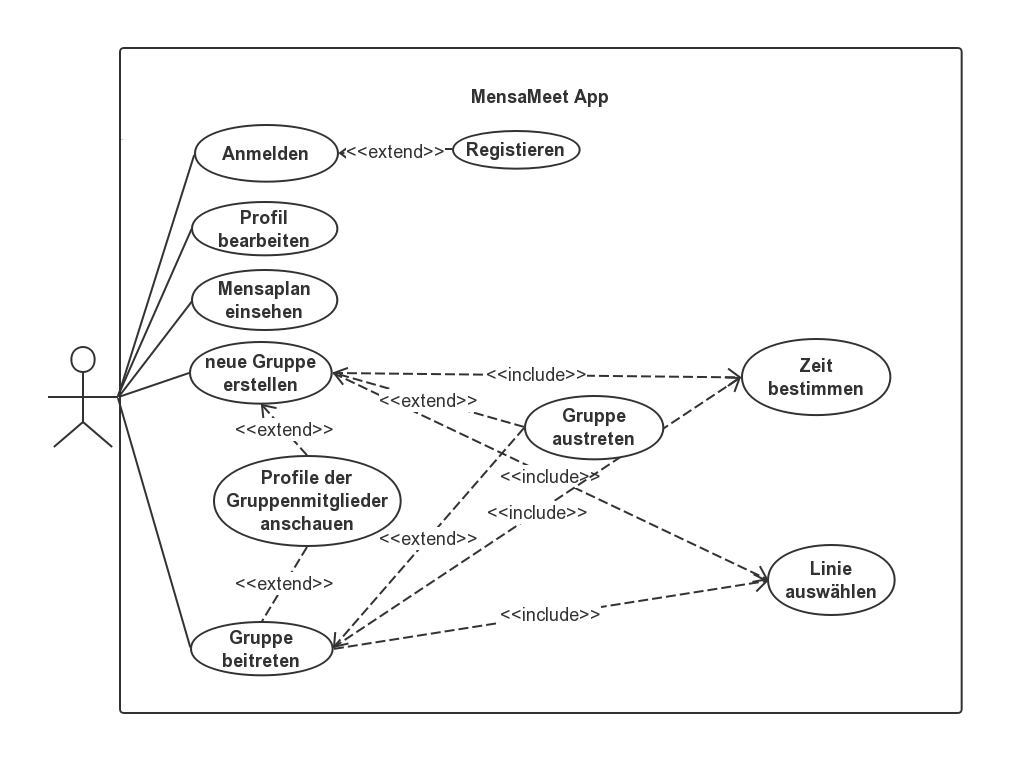
\includegraphics[scale=0.5]{useCase_MensaMeet.jpg}
\end{center}

\chapter{Glossar}
 \begin{itemize}
 \item \hypertarget{label1}{Mensabesucher}: Personen, die in der Mensa essen möchten und dürfen. Also Studenten, Professoren, wissenschaftliche Mitarbeiter des KITs, Auszubildende am KIT, Schüler
 \item \hypertarget{label2}{Gruppenparameter}: Hierzu zählen alle folgenden Angaben, die zum Erstellen einer Gruppe nötig sind: Ein eindeutiger Grupenname, ein Motto, genau eine Mensalinie bzw. ein Mensawerk, der Treffzeitpunkt, die maximale Gruppengröße.
\item \hypertarget{label3}{Essensplanung}: Zur Essensplanung an der Mensa müssen folgende Fragen geklärt werden: Welches Angebot gibt es?, An welchen Mensalinien/-werken würde ich essen?, Um wie viel Uhr möchte ich essen? 
  
 \end{itemize}
 


\end{document}
